
%%%%%%%%%%%%%%%%%%%%%%%%%%%%%%%%%%%%%%%%%%%%%%%%%%%%%%%%%%%%%%%%%%%%%%%%%
%%%%%%%%%%%%%%%%%%%%%%%%%%%%%%%%%%%%%%%%%%%%%%%%%%%%%%%%%%%%%%%%%%%%%%%%%
%%%%%%%%%%%%%%%%%%%%%%%%%%%%%%%%%%%%%%%%%%%%%%%%%%%%%%%%%%%%%%%%%%%%%%%%%

\begin{frame}{What makes an estimator non-robust?  A tail sum.}
% Report non-robustness if
%
\begin{align*}
%
%\textrm{Report non-robustness if }
\Delta \le{}& \thetafunlin(\w^*) - \thetafun(\thetahat)
        & \textrm{Report non-robustness}
    \\=&{} -\sum_{n=1}^{\lfloor \alpha N \rfloor} \infl_{(n)}
        & \textrm{(By definition)}
    \\=&{} -\frac{1}{N} \sum_{n=1}^{\lfloor \alpha N \rfloor} N \infl_{(n)}
        & \textrm{(Recall }\infl_n = O_p(N^{-1})\textrm{)}
    % \\=&{} -\meann \ind{n \le \lfloor \alpha N \rfloor} N \infl_{(n)}
    %     & \textrm{(By definition)}
    \\\le&{}
        \underbrace{
            \left( \meann N^2 \infl_{(n)}^2 \right)^{1/2}
        }_{\displaystyle =: \noise}
        \underbrace{
            \left( \meann \ind{n \le \lfloor \alpha N \rfloor} \right)^{1/2}
        }_{\displaystyle =: \shape \le \sqrt{\alpha}}
        & \textrm{(Cauchy-Schwartz)}
    % \\\le&{} \left( \meann N^2 \infl_{(n)}^2 \right)^{1/2} \sqrt{\alpha}
%
\end{align*}
%
Suppose that $\thetahat \plim \theta_0$ and $\thetafun(\thetahat)
\rightsquigarrow \mathcal{N}(\thetafun(\theta_0), \sigma^2)$.

Typically, $\noise \plim \sigma$ \citep{hampel1986robustbook}.

A slightly more careful analysis gives $\shape \le \sqrt{\alpha(1-\alpha)}$.

% (Using $\sumn \infl_n = 0$).

\end{frame}



%%%%%%%%%%%%%%%%%%%%%%%%%%%%%%%%%%%%%%%%%%%%%%%%%%%%%%%%%%%%%%%%%%%%%%%%%
%%%%%%%%%%%%%%%%%%%%%%%%%%%%%%%%%%%%%%%%%%%%%%%%%%%%%%%%%%%%%%%%%%%%%%%%%
%%%%%%%%%%%%%%%%%%%%%%%%%%%%%%%%%%%%%%%%%%%%%%%%%%%%%%%%%%%%%%%%%%%%%%%%%

\begin{frame}{What makes an estimator non-robust?  A tail sum.}

Report non-robustness if the \textbf{``signal to noise ratio''}
$\frac{\Delta}{\noise} \le \shape$ where

% Report non-robustness if
% $ \Delta \le
%   -\sum_{n=1}^{\lfloor \alpha N \rfloor} \infl_{(n)}$
% \onslide<5->{
% $= \noise \shape$ where
% }
%
\begin{itemize}
\item The ``noise'' $\noise^2 \rightarrow \mathrm{Var}(\sqrt{N}\phi)$
    \citep{hampel1986robustbook}
\item The ``shape'' $\shape \le \sqrt{\alpha (1 - \alpha)}$
    and converges to a nonzero constant
\end{itemize}

\begin{center}
\begin{minipage}{0.85\linewidth}
\begin{tikzpicture}
    \onslide<1->{
    \node[anchor=south west,inner sep=0] (image) at (0,0) {
        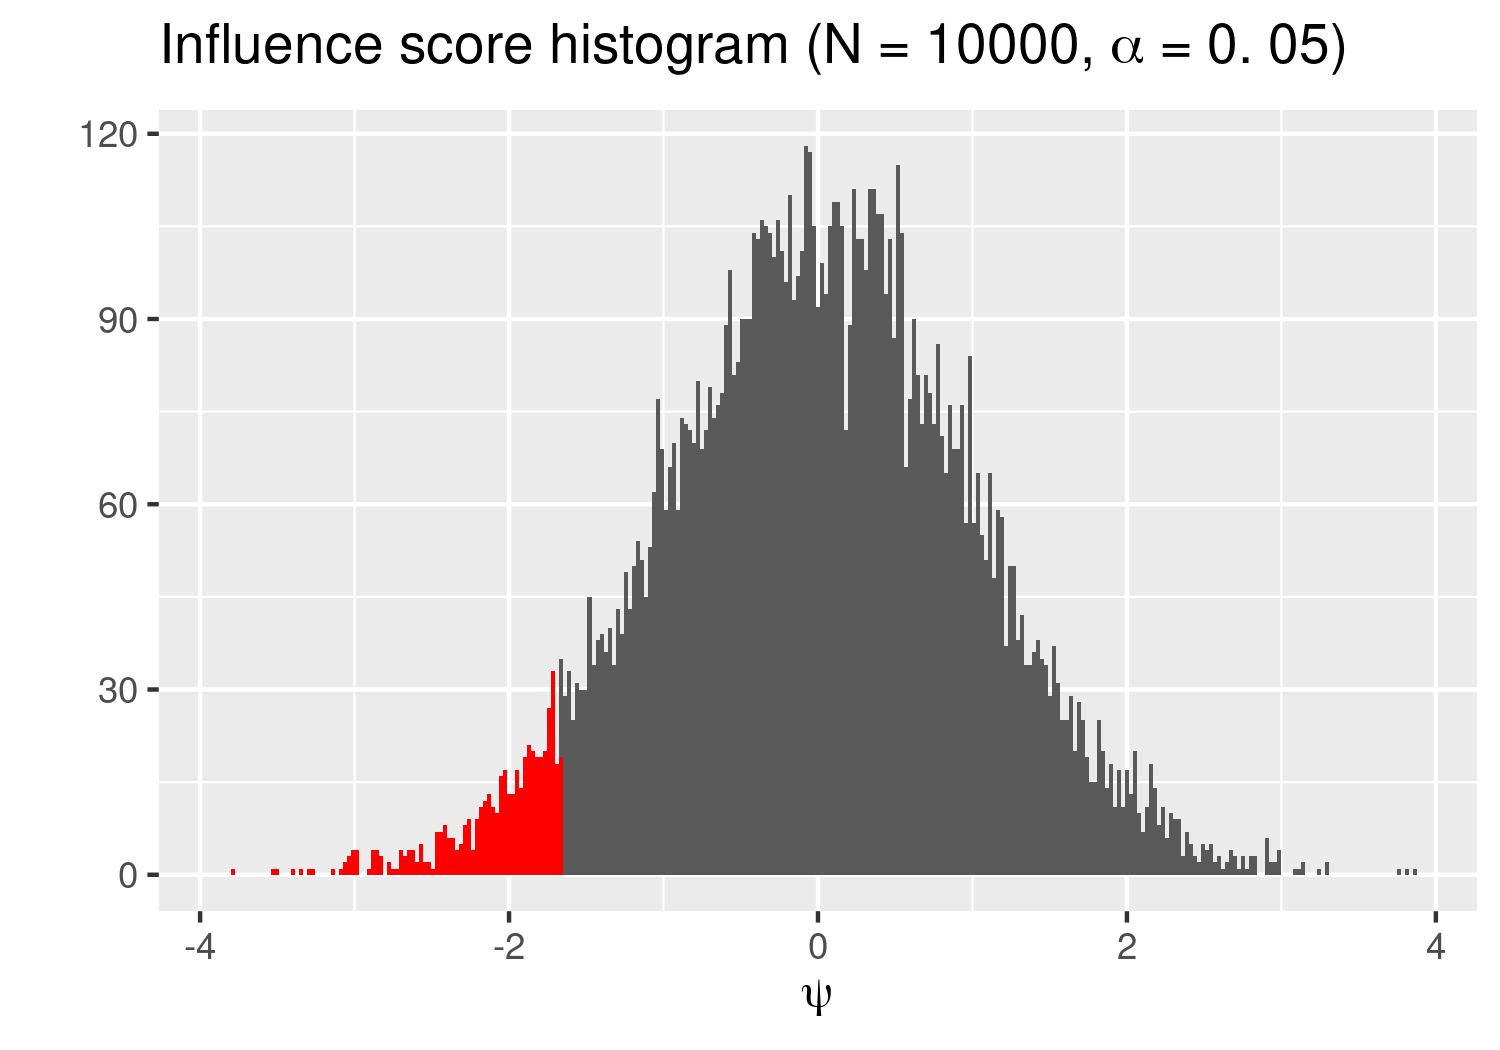
\includegraphics[width=0.98\textwidth]{static_figures/simple_infl_example.png}
    };
    }
    \onslide<1->{
    \begin{scope}[x={(image.south east)},y={(image.north west)}]
        \draw [stealth-stealth][thick][yellow](0.44, 0.4) -- (0.64, 0.4);
    \end{scope}
    \begin{scope}[x={(image.south east)},y={(image.north west)}]
        \draw (0.55,0.38) node[below,yellow][text width=3cm][align=center]
        {\small $\noise$ is controlled by $\var{}{\sqrt{N}\phi(\thetahat)}$};
    \end{scope}
    }
    \onslide<1->{
    \begin{scope}[x={(image.south east)},y={(image.north west)}]
        \draw [stealth-][thick][red](0.3, 0.25) -- (0.3, 0.5);
    \end{scope}
    \begin{scope}[x={(image.south east)},y={(image.north west)}]
        \draw (0.3, 0.5) node[above,red][text width=3cm][align=center]
        {\small $\shape$ is (roughly) controlled by Cauchy-Schwartz};
    \end{scope}
    }
\end{tikzpicture}
\end{minipage}
\end{center}

\end{frame}


%%%%%%%%%%%%%%%%%%%%%%%%%%%%%%%%%%%%%%%%%%%%%%%%%%%%%%%%%%%%%%%%%%%%%%%%%
%%%%%%%%%%%%%%%%%%%%%%%%%%%%%%%%%%%%%%%%%%%%%%%%%%%%%%%%%%%%%%%%%%%%%%%%%
%%%%%%%%%%%%%%%%%%%%%%%%%%%%%%%%%%%%%%%%%%%%%%%%%%%%%%%%%%%%%%%%%%%%%%%%%

\begin{frame}{Corollaries.}

% {\small
% \textbf{Key quantities:}\\
% \pause $\alpha$  = The proportion of left out points\\
% \pause $\Delta$  = The signal = The change in $\phi$ that would alter your
% conclusion\\
% \pause $\noise^2$ = The noise = A consistent estimator of
% $\mathrm{Var}(\sqrt{N}\phi)$\\
% \pause $\shape$ =
%     The shape = Converges to a nonzero constant, $\le \sqrt{\alpha(1-\alpha)}$\\
% }

\pause
Report non-robustness if the \textbf{``signal to noise ratio''}
$\frac{\Delta}{\noise} \le \shape$.

\hrulefill

%\vspace{-1em}

\pause
\vspace{0.5em}
\textbf{Corollary:  Non-robustness possible even with correct specification.}
\vspace{-0.4em}
% {\small The noise $\noise$ may be larger than the effect
% $\Delta$ you're trying to measure.}

\pause
\vspace{0.5em}
\textbf{Corollary:  Leave-$\lfloor \alpha N \rfloor$-out robustness does not vanish as $N \rightarrow \infty$.}
% \vspace{-0.4em}
%
% Both $\shape$ and $\noise$ typically converge to nonzero constants.

\pause
\vspace{0.5em}
Recall that standard errors reject when
$\frac{\Delta}{\noise} \le \frac{1.96}{\sqrt{N}}$.

\pause
\vspace{0.5em}
\textbf{Corollary:  Leave-$\lfloor \alpha N \rfloor$-out is different from standard errors.}
%\vspace{-0.4em}
% $1.96 / \sqrt{N} \ne \shape$

\pause
\vspace{0.5em}
\textbf{Corollary:  Insignificance is always non-robust.}
\vspace{-0.4em}

Take $\Delta = \frac{1.96 \hat \sigma_\phi}{\sqrt{N}} \rightarrow 0 \le
\shape$.

\pause
\vspace{0.5em}
\textbf{Corollary:  Gross outliers primarily affect robustness
through $\noise$.}
\vspace{-0.4em}
Cauchy-Schwartz is tight when all the influence scores are the same.

\end{frame}
